\documentclass{article}
\usepackage{graphicx} % Required for inserting images
% header

%% natbib
\usepackage{natbib}
\bibliographystyle{plain}

%% comment
\usepackage{comment}

% no automatic indentation
\usepackage{indentfirst}

% manually indent
\usepackage{xargs} % \newcommandx
\usepackage{calc} % calculation
\newcommandx{\tab}[1][1=1]{\hspace{\fpeval{#1 * 10}pt}}
% \newcommand[number of parameters]{output}
% \newcommandx[number of parameters][parameter index = x]{output}
% use parameter index = x to substitute the default argument
% use #1, #2, ... to get the first, second, ... arguments
% \tab for indentation
% \tab{2} for for indentation twice

% note
\newcommandx{\note}[1]{\textit{\textcolor{red}{#1}}}
\newcommand{\todo}{\note{TODO}}
% \note{TODO}

%% math package
\usepackage{amsfonts}
\usepackage{amsmath}
\usepackage{amssymb}
\usepackage{tikz-cd}
\usepackage{mathtools}
\usepackage{amsthm}

%% operator
\DeclareMathOperator{\tr}{tr}
\DeclareMathOperator{\diag}{diag}
\DeclareMathOperator{\sign}{sign}
\DeclareMathOperator{\grad}{grad}
\DeclareMathOperator{\curl}{curl}
\DeclareMathOperator{\Div}{div}
\DeclareMathOperator{\card}{card}
\DeclareMathOperator{\Span}{span}
\DeclareMathOperator{\real}{Re}
\DeclareMathOperator{\imag}{Im}
\DeclareMathOperator{\supp}{supp}
\DeclareMathOperator{\im}{im}
\DeclareMathOperator{\aut}{Aut}
\DeclareMathOperator{\inn}{Inn}
\DeclareMathOperator{\Char}{char}
\DeclareMathOperator{\Sylow}{Syl}
\DeclareMathOperator{\coker}{coker}
\DeclareMathOperator{\inc}{in}
\DeclareMathOperator{\Sd}{Sd}
\DeclareMathOperator{\Hom}{Hom}
\DeclareMathOperator{\interior}{int}
\DeclareMathOperator{\ob}{ob}
\DeclareMathOperator{\Set}{Set}
\DeclareMathOperator{\Top}{Top}
\DeclareMathOperator{\Meas}{Meas}
\DeclareMathOperator{\Grp}{Grp}
\DeclareMathOperator{\Ab}{Ab}
\DeclareMathOperator{\Ch}{Ch}
\DeclareMathOperator{\Fun}{Fun}
\DeclareMathOperator{\Gr}{Gr}
\DeclareMathOperator{\End}{End}
\DeclareMathOperator{\Ad}{Ad}
\DeclareMathOperator{\ad}{ad}
\DeclareMathOperator{\Bil}{Bil}
\DeclareMathOperator{\Skew}{Skew}
\DeclareMathOperator{\Tor}{Tor}
\DeclareMathOperator{\Ho}{Ho}
\DeclareMathOperator{\RMod}{R-Mod}
\DeclareMathOperator{\Ev}{Ev}
\DeclareMathOperator{\Nat}{Nat}
\DeclareMathOperator{\id}{id}
\DeclareMathOperator{\Var}{Var}
\DeclareMathOperator{\Cov}{Cov}
\DeclareMathOperator{\RV}{RV}
\DeclareMathOperator{\rank}{rank}

%% pair delimiter
\DeclarePairedDelimiter{\abs}{\lvert}{\rvert}
\DeclarePairedDelimiter{\inner}{\langle}{\rangle}
\DeclarePairedDelimiter{\tuple}{(}{)}
\DeclarePairedDelimiter{\bracket}{[}{]}
\DeclarePairedDelimiter{\set}{\{}{\}}
\DeclarePairedDelimiter{\norm}{\lVert}{\rVert}

%% theorems
\newtheorem{axiom}{Axiom}
\newtheorem{definition}{Definition}
\newtheorem{theorem}{Theorem}
\newtheorem{proposition}{Proposition}
\newtheorem{corollary}{Corollary}
\newtheorem{lemma}{Lemma}
\newtheorem{remark}{Remark}
\newtheorem{claim}{Claim}
\newtheorem{problem}{Problem}
\newtheorem{assumption}{Assumption}
\newtheorem{example}{Example}
\newtheorem{exercise}{Exercise}

%% empty set
\let\oldemptyset\emptyset
\let\emptyset\varnothing

\newcommand\eps{\epsilon}

% mathcal symbols
\newcommand\Tau{\mathcal{T}}
\newcommand\Ball{\mathcal{B}}
\newcommand\Sphere{\mathcal{S}}
\newcommand\bigO{\mathcal{O}}
\newcommand\Power{\mathcal{P}}
\newcommand\Str{\mathcal{S}}


% mathbb symbols
\usepackage{mathrsfs}
\newcommand\N{\mathbb{N}}
\newcommand\Z{\mathbb{Z}}
\newcommand\Q{\mathbb{Q}}
\newcommand\R{\mathbb{R}}
\newcommand\C{\mathbb{C}}
\newcommand\F{\mathbb{F}}
\newcommand\T{\mathbb{T}}
\newcommand\Exp{\mathbb{E}}

% mathrsfs symbols
\newcommand\Borel{\mathscr{B}}

% algorithm
\usepackage{algorithm}
\usepackage{algpseudocode}

% longproof
\newenvironment{longproof}[1][\proofname]{%
  \begin{proof}[#1]$ $\par\nobreak\ignorespaces
}{%
  \end{proof}
}


% for (i) enumerate
% \begin{enumerate}[label=(\roman*)]
%   \item First item
%   \item Second item
%   \item Third item
% \end{enumerate}
\usepackage{enumitem}

% insert url by \url{}
\usepackage{hyperref}

% margin
\usepackage{geometry}
\geometry{
a4paper,
total={190mm,257mm},
left=10mm,
top=20mm,
}



\title{ma4261\_hw1}
\author{Nguyen Ngoc Khanh - A0275047B}
\date{August 2024}

\begin{document}

\maketitle

\section{Problem 1}
Consider random variables $X$ and $Y$ such that $Y$ is uniformly distributed over $\mathcal{Y} = \set{0, 1}^b$. Let $\hat{Y}$ be an estimate of $Y$ obtained by observing $X$. Show that
$$
    Pr(\hat{Y} \neq Y) \geq 1 - \frac{I(X; Y) + 1}{b}
$$

Now, suppose that $X_1, X_2, ..., X_n, Y$ are random variables such that $X_1, X_2, ..., X_n$ are mutually independent and $Y$ is as before. For each $i \in [n]$, let $\hat{Y}_i$ denote an estimate of $Y$ obtained from observing $X_i$. Show that
$$
    \max_{1 \leq i \leq n} Pr(\hat{Y}_i \neq Y) \geq 1 - \frac{1}{n} - \frac{1}{b}
$$

\subsection{$P(\hat{Y} \neq Y)$}

By Fano inequality, we have
\begin{align*}
    Pr(\hat{Y} \neq Y)
    &\geq \frac{H(Y|X) - 1}{\log \abs{\mathcal{Y}}} \\
    &= \frac{H(Y) - I(X; Y) - 1}{\log \abs{\mathcal{Y}}} \\
    &= \frac{\log \abs{\mathcal{Y}} - I(X; Y) - 1}{\log \abs{\mathcal{Y}}} &\text{($Y$ uniform)}\\
    &= 1 - \frac{I(X; Y) + 1}{\log \abs{\mathcal{Y}}} \\
    &= 1 - \frac{I(X; Y) + 1}{b} &\text{($\abs{\mathcal{Y}} = 2^b$)} \\
\end{align*}

\subsection{$\max_{1 \leq i \leq n} Pr(\hat{Y}_i \neq Y)$}

By Fano inequality, for each $i \in [n]$
$$
    Pr(\hat{Y}_i \neq Y) \geq 1 - \frac{I(X_i; Y)}{b} - \frac{1}{b}
$$

Then,

$$
    \max_{1 \leq i \leq n} Pr(\hat{Y}_i \neq Y) \geq \frac{1}{n} \sum_{i=1}^n Pr(\hat{Y}_i \neq Y) \geq 1 - \frac{\sum_{i=1}^n I(X_i; Y)}{nb} - \frac{1}{b}
$$

We will show that $- \frac{\sum_{i=1}^n I(X_i; Y)}{nb} \geq - \frac{1}{n}$, that is $\sum_{i=1}^n I(X_i; Y) \leq b$. Indeed, as $X_1, X_2, ..., X_n$ are independent

$$
    \sum_{i=1}^n I(X_i; Y) = I(X_1^n; Y)
$$

Hence

$$
    \sum_{i=1}^n I(X_i; Y) = I(X_1^n; Y) = H(Y) - H(Y|X_1^n) \leq H(Y) = b
$$

\begin{lemma}
If $X, Z$ are independent, then
$$
    I(X, Z; Y) = I(X; Y) + (Z; Y)
$$
\begin{proof}
    $
        I(X, Z; Y) = H(X, Z) - H(X, Z | Y) = (H(X) + H(Z)) - (H(X|Y) + H(Z|Y)) = I(X; Y) + (Z; Y)
    $
\end{proof}
\end{lemma}

\section{Problem 2}
Let $L_\eps(X)$ be defined as the minimum length of a source code designed for source $X \sim p_X$ with error probability $\eps$, i.e.
$$
    L_\eps(X) = \inf \set{\log M: \exists (1, M)-\text{source code with } P_e \leq \eps}
$$

\begin{enumerate}
\item Show that if there exists a $\lambda$ such that $Pr(-\log p_X(X) \leq \lambda) \geq 1 - \eps$, then $L_\eps(X) \leq \lambda$

\item A common qualification of randomness, besides the entropy is the  Rényi entropy of order $\alpha \in (0, 1) \cup (1, \infty)$ defined by
$$
    H_\alpha(X) = \frac{1}{1 - \alpha} \log \sum_{x \in \mathcal{X}} p_X(x)^\alpha
$$

Show that $\lim_{\alpha \to 1} H_\alpha(X) = H(X)$

\item Show that for fixed $p_X$, the map $\alpha \mapsto H_\alpha(X)$ is non-increasing

\item Prove that for every $\alpha \in (0, 1)$ and $\eps > 0$
$$
    L_\eps(X) \leq H_\alpha(X) + \frac{1}{1-\alpha} \log \frac{1}{\eps} + 1
$$

\item Prove that for every $\beta > 1$ and $\delta \in (0, 1-\eps)$
$$
    L_\eps(X) \geq H_\beta(X) - \frac{1}{\beta-1} \log \frac{1}{\delta} - \log \frac{1}{1-\eps-\delta}
$$

\item Show that if $X^n = (X_1, X_2, ..., X_n)$ consists of i.i.d random variables $X \sim p_X$, then $H_\alpha(X^n) = n H_\alpha(X)$ for all $\alpha > 0$

\item Use the above parts to prove fixed-to-fixed length source coding theorem with strong converse, i.e. you should provide bounds on
$$
    \liminf_{n \to \infty} \frac{1}{n} L_\eps(X^n) \text{ and } \limsup_{n \to \infty} \frac{1}{n} L_\eps(X^n)
$$
\end{enumerate}

\subsection{if there exists a $\lambda$ such that $Pr(-\log p_X(X) \leq \lambda) \geq 1 - \eps$, then $L_\eps(X) \leq \lambda$}

Let 
$$
    A_\lambda = \set*{x \in \mathcal{X}: -\log p_X(x) \leq \lambda} \subseteq \mathcal{X}
$$
    
Given $P(A_\lambda) \geq 1 - \eps$, we will upper bound the size of $A_\lambda$ so that there is a code that map $A_\lambda$ injectively into $M$ code words.

If $x \in A_\lambda$, then
\begin{align*}
    -\log p_X(x) &\leq \lambda \\
    \log p_X(x) &\leq -\lambda \\
    p_X(x) &\geq 2^{-\lambda}
\end{align*}


Moreover, 
\begin{align*}
    1
    &= \sum_{x \in \mathcal{X}} p_X(x) \\
    &\geq \sum_{x \in A_\lambda} p_X(x) &\text{($A_\lambda \subseteq \mathcal{X}$)}\\
    &\geq \sum_{x \in A_\lambda} 2^{-\lambda} &\text{($x \in A_\lambda \implies p_X(x) \geq 2^{-\lambda}$)}\\
    &= 2^{-\lambda} |A_\lambda|
\end{align*}

Then, $|A_\lambda| \leq 2^\lambda$. Let $M = 2^\lambda$, there exists an injective map from $A_\lambda$ into $[M] = \set{1, ..., M}$. As $P(A_\lambda) \geq 1 - \eps$, $P_e < \eps$, hence, $L_\eps(X) \leq \log M = \lambda$

\subsection{$\lim_{\alpha \to 1} H_\alpha(X) = H(X)$}

Let $f(\alpha) = \log \sum_{x \in \mathcal{X}} p_X(x)^\alpha$, $f$ is analytic on $(0, \infty)$, we have ($\log$ denotes $\log_2$)

$$
    f'(\alpha) = \frac{1}{\sum_{x \in \mathcal{X}} p_X(x)^\alpha} \sum_{x \in \mathcal{X}} p_X(x)^\alpha \log p_X(x)
$$

Let $g(\alpha) = \frac{1}{1-\alpha}$, $g$ is analytic on $\R \setminus \set{1}$, we have

$$
    g'(\alpha) = \frac{1}{(1-\alpha)^2}
$$

Write $\alpha \mapsto f(\alpha)$ as a Taylor series around $\alpha=1$, and note that as $f$ is analytic around $1$, $f^{(n)}(1)$ is finite for all $n$, then

$$
    f(\alpha) = f(1) + f'(1) (\alpha - 1) + o(\alpha - 1)
$$

where $\frac{o(\alpha - 1)}{\alpha - 1} \to 0$ as $\alpha \to 1$. Therefore, around $\alpha=1$
\begin{align*}
    H_\alpha(X)
    &= g(\alpha) f(\alpha) \\
    &= \frac{1}{1-\alpha} (f(1) + f'(1) (\alpha - 1) + o(\alpha - 1)) \\
    &= f(1) + f'(1) + \frac{o(\alpha - 1)}{\alpha - 1}
\end{align*}

Hence,
$$
    \lim_{\alpha \to 1} H_\alpha(X) = f(1) + f'(1) = H(X)
$$

\subsection{for fixed $p_X$, the map $\alpha \mapsto H_\alpha(X)$ is non-increasing}

For any $\alpha \in (0, 1) \cup (1, \infty)$,
$$
    \frac{d}{d\alpha} H_\alpha(X) = g'(\alpha) f(\alpha) + g(\alpha) f'(\alpha)
$$

Note that $g'(\alpha) = \frac{1}{(1 - \alpha)^2} > 0$, we will show that $ - f(\alpha) - \frac{g(\alpha)}{g'(\alpha)} f'(\alpha) \geq 0$ for all $\alpha \in (0, 1) \cup (1, \infty)$, let $s = \sum_{x \in \mathcal{X}} p_X(x)^\alpha$

\begin{align*}
    - f(\alpha) - \frac{g(\alpha)}{g'(\alpha)} f'(\alpha)
    &= - \log s + (\alpha - 1) \frac{\sum_{x \in \mathcal{X}} p(x)^\alpha \log p(x)}{s} \\
    &= - \log s + \frac{1}{s} \sum_{x \in \mathcal{X}} (\alpha - 1) p(x)^\alpha \log p(x) \\
    &= \tuple*{\frac{1}{s} \sum_{x \in \mathcal{X}} - p(x)^\alpha \log s} + \tuple*{\frac{1}{s} \sum_{x \in \mathcal{X}} p(x)^\alpha \log p(x)^\alpha -  p(x)^\alpha \log p(x)} \\
    &= \frac{1}{s} \sum_{x \in \mathcal{X}} p(x)^\alpha [- (\log s) + \log p(x)^\alpha - \log p(x)] \\
    &= \sum_{x \in \mathcal{X}} \frac{p(x)^\alpha}{s} \log \frac{p(x)^\alpha / s}{p(x)} \\
    &= \sum_{x \in \mathcal{X}} q(x) \log \frac{q(x)}{p(x)} &\text{(where $q(x) = \frac{p(x)^\alpha}{s}$)} \\
    &= D(q || p) \geq 0 &\text{($q$ is a distribution on $\mathcal{X}$)}
\end{align*}

\subsection{for every $\alpha \in (0, 1)$ and $\eps > 0$, $L_\eps(X) \leq H_\alpha(X) + \frac{1}{1-\alpha} \log \frac{1}{\eps} + 1$}

Let 
$$
    A_\alpha = \set*{x \in \mathcal{X}: - \log p(x) \leq H_\alpha(X) + \frac{1}{1-\alpha} \log \frac{1}{\eps}}
$$

If $x \notin A_\alpha$, then 
\begin{align*}
    - \log p(x) &> H_\alpha(X) + \frac{1}{1-\alpha} \log \frac{1}{\eps} \\
    \log p(x) &< -H_\alpha(X) + \frac{1}{1-\alpha} \log \eps \\
    p(x) &< 2^{-H_\alpha(X)} \eps^{1/(1-\alpha)} \\
    p(x)^{1 - \alpha} &< \eps 2^{-(1-\alpha) H_\alpha(X)} &\text{($1 - \alpha > 0$)}
\end{align*}

Then
\begin{align*}
    P(A_\alpha^C)
    &= \sum_{x \notin A_\alpha} p(x) \\
    &= \sum_{x \notin A_\alpha} p(x)^{1-\alpha} p(x)^\alpha \\
    &< \eps 2^{-(1-\alpha) H_\alpha(X)} \sum_{x \notin A_\alpha} p(x)^\alpha  \\
    &\leq \eps 2^{-(1-\alpha) H_\alpha(X)} \sum_{x \in \mathcal{X}} p(x)^\alpha \\
    &= \eps 2^{-(1-\alpha) H_\alpha(X)} 2^{(1-\alpha) H_\alpha(X)} = \eps\\
\end{align*}

Hence, $P(A_\alpha) \geq 1 - \eps$, from (1) we have $L_\eps(X) \leq H_\alpha(X) + \frac{1}{1-\alpha} \log \frac{1}{\eps} < H_\alpha(X) + \frac{1}{1-\alpha} \log \frac{1}{\eps} + 1$.
\subsection{for every $\beta > 1$ and $\delta \in (0, 1-\eps)$
$
    L_\eps(X) \geq H_\beta(X) - \frac{1}{\beta-1} \log \frac{1}{\delta} - \log \frac{1}{1-\eps-\delta}
$}

\begin{lemma}[Han-Verdú]
    \label{lemma3}
    If there exists $\lambda$ such that $Pr(- \log p(X) \geq \lambda) \geq 1 - \delta$, then $L_\eps(X) \geq \lambda - \log \frac{1}{1 - \eps - \delta}$
\end{lemma}

\begin{proof}[Proof of Lemma \ref{lemma3}]

Suppose, there is a code of length $L$ with error probability $P_e \leq \eps$. Let 
\begin{align*}
    T &= \set{x \in \mathcal{X}: - \log p(X) \geq \lambda} = \set{x \in \mathcal{X}: p(X) \leq 2^{-\lambda}}\\
    S &= \set{x \in \mathcal{X}: \phi f x = x}
\end{align*}

Then, 

\begin{align*}
    P(T) 
    &= P(T \cap S^C) + P(T \cap S) \\
    &\leq P(S^C) + P(T \cap S) \\
    &= P_e + P(T \cap S) \\
    &\leq \eps + P(T \cap S) \\
    &= \eps + \sum_{x \in T \cap S} p(x) \\
    &\leq \eps + 2^{-\lambda} |T \cap S| \\
    &\leq \eps + 2^{-\lambda} |S| \\
\end{align*}

$S$ is the set that is decoded correctly, so the map $f: S \to [2^L]$ is injective, hence $|S| \leq 2^L$. Therefore, 
$$
    1 - \delta \leq P(T) \leq \eps + 2^{-\lambda}|S| \leq \eps + 2^{-\lambda + L}
$$

Then $L \geq \lambda - \log \frac{1}{1 - \eps - \delta}$, hence

$$
    L_\eps(X) \geq \lambda - \log \frac{1}{1 - \eps - \delta}
$$

\end{proof}

\begin{proof}[Main Proof]
Let
$$
    B_\beta = \set*{x \in \mathcal{X}: -\log p(X) \geq H_\beta(X) - \frac{1}{\beta-1} \log \frac{1}{\delta}}
$$

If $x \notin B_\beta$, then
\begin{align*}
    -\log p(x) &< H_\beta(X) - \frac{1}{\beta-1} \log \frac{1}{\delta} \\
    \log p(x) &> - H_\beta(X) + \frac{1}{1-\beta} \log \delta \\
    p(x) &> 2^{- H_\beta(X)} \delta^{1/(1 - \beta)} \\
    p(x)^{1-\beta} &< \delta 2^{- (1-\beta) H_\beta(X)} &\text{($1 - \beta < 0$)}\\
\end{align*}

Then
\begin{align*}
    P(B_\beta^C)
    &= \sum_{x \notin B_\beta} p(x) \\
    &= \sum_{x \notin B_\beta} p(x)^{1-\beta} p(x)^\beta \\
    &< \delta 2^{- (1-\beta) H_\beta(X)} \sum_{x \notin B_\beta} p(x)^\beta \\
    &\leq \delta 2^{- (1-\beta) H_\beta(X)} \sum_{x \in \mathcal{X}} p(x)^\beta \\
    &= \delta 2^{- (1-\beta) H_\beta(X)} 2^{(1-\beta)H_\beta(X)} = \delta \\
\end{align*}

Hence, $P(B_\beta) \geq 1 - \delta$, from Lemma \ref{lemma3}, we have $L_\eps(X) \leq H_\beta(X) - \frac{1}{\beta-1} \log \frac{1}{\delta} - \log \frac{1}{1-\eps-\delta}$
    
\end{proof}



\subsection{if $X^n = (X_1, X_2, ..., X_n)$ consists of i.i.d random variables $X \sim p_X$, then $H_\alpha(X^n) = n H_\alpha(X)$ for all $\alpha > 0$}

\begin{lemma}
\label{lemma4}
If $X, Y$ are independent, then $H_\alpha(X,Y) = H_\alpha(X) + H_\alpha(Y)$
\begin{proof}[Proof of Lemma \ref{lemma4}]
    \begin{align*}
        H_\alpha(X,Y)
        &= \frac{1}{1-\alpha} \log \sum_{x \in \mathcal{X}} \sum_{y \in \mathcal{Y}} p_{X,Y}(x, y)^\alpha \\
        &= \frac{1}{1-\alpha} \log \sum_{x \in \mathcal{X}} \sum_{y \in \mathcal{Y}} p_{X}(x)^\alpha p_Y(y)^\alpha &\text{(independent)}\\
        &= \frac{1}{1-\alpha} \log \bracket*{\tuple*{\sum_{x \in \mathcal{X}} p_{X}(x)^\alpha} \tuple*{\sum_{y \in \mathcal{Y}}  p_Y(y)^\alpha}} \\
        &= \frac{1}{1-\alpha} \bracket*{\log \tuple*{\sum_{x \in \mathcal{X}} p_{X}(x)^\alpha} + \log \tuple*{\sum_{y \in \mathcal{Y}}  p_Y(y)^\alpha}} \\
        &= H_\alpha(X) + H_\alpha(Y)
    \end{align*}
\end{proof}
\end{lemma}

\begin{proof}[Main Proof]
    Generalize from the case of two variables
\end{proof}

\subsection{prove the fixed-to-fixed-length source coding theorem with strong converse}

Fix $0 < \alpha < 1 < \beta$, $\eps, \delta$, we have

$$
    H_\beta(X) + \frac{1}{n} \tuple*{- \frac{1}{\beta-1} \log \frac{1}{\delta} - \log \frac{1}{1-\eps-\delta}} \leq \frac{1}{n} L_\eps(X^n) \leq H_\alpha(X) + \frac{1}{n}\tuple*{\frac{1}{1-\alpha} \log \frac{1}{\eps} + 1}
$$

Therefore, 

$$
    H_\beta(X) \leq \liminf_{n \to \infty} \frac{1}{n} L_\eps(X^n) \leq \limsup_{n \to \infty} \frac{1}{n} L_\eps(X^n) \leq H_\alpha(X)
$$

As $H_\beta(X) \to H(X)$ as $\beta \to 1^+$ and $H_\alpha(X) \to H(X)$ as $\alpha \to 1^-$, therefore $\lim_{n \to \infty} \frac{1}{n} L_\eps(X^n)$ exists and 
$$
    \lim_{n \to \infty} \frac{1}{n} L_\eps(X^n) = H(X)
$$

for all $\eps \in (0, 1)$ (strong converse)

\section{Problem 3}
An $n \times n$ non-negative matrix $W = [W_{ij}]$ is called doubly stochastic if $\sum_{i} W_{ij} = 1$ and for all $j$ and $\sum_{j} W_{ij} = 1$ for all $i$

\begin{enumerate}
\item Let $p = (p_1, p_2, ..., p_n)$ be a probability vector, i.e. $p_i \geq 0$ for all $i$ and $\sum_{i} p_i = 1$. Let $q = pW$ where $W$ is doubly stochastic. Show that $q$ is a probability vector and $H(q) \geq H(p)$.

\item Show that stationary distribution $\mu$ for a doubly stochastic matrix $W$ is the uniform distribution

\item Conversely, prove that if uniform distribution is a stationary distribution for a Markov transition matrix $W$, then $W$ is doubly stochastic.
\end{enumerate}

\subsection{$q$ is a probability vector and $H(q) \geq H(p)$}

Entries of $W$ and $p$ are non-negative, hence entries of $q$ are non-negative. Let $1 = (1, 1, ..., 1) \in \R^n$ be a row vector. We will show that $q 1^T = 1$, that is the sum of entries of $q$ is $1$.

\begin{align*}
    q 1^T
    &= p W 1^T \\
    &= p 1^T &\text{(sum of each row of $W$ is $1$)} \\
    &= 1 &\text{(sum of entries of $p$ is $1$)}
\end{align*}

\subsection{stationary distribution $\mu$ for a doubly stochastic matrix $W$ is the uniform distribution}

As sum of each column of $W$ is $1$, $1 W = 1$, therefore, $\mu = \tuple*{\frac{1}{n}, \frac{1}{n}, ..., \frac{1}{n}}$ being a uniform distribution is a left eigen vector of $W$, i.e. a stationary distribution

\subsection{if uniform distribution is a stationary distribution for a Markov transition matrix $W$, then $W$ is doubly stochastic}

Markov transition matrix has sum of each row is $1$, furthermore, $\mu = \tuple*{\frac{1}{n}, \frac{1}{n}, ..., \frac{1}{n}}$ is stationary distribution, i.e. a left eigen vector of eigen value $1$. Hence, $1 W = 1$, that is equivalent to sum of each column of $W$ is $1$, therefore, $W$ is doubly stochastic

\section{Problem 4}
Consider a discrete memoryless source $X$ with alphabet $\set{1, 2, ..,, M}$. Suppose that the symbol probabilities are ordered and satisfy $p_1 > p_2 > ... > p_M$ and also satisfy $p_1 < p_{M-1} + p_M$. Let $l_1, l_2, ..., l_M$ be the length of prefix-free code of minimum expected length for such a source.
\begin{enumerate}
\item TRUE or FALSE: $l_1 \leq l_2 \leq ... \leq l_M$. Provide a short justification

\item Show that if Huffman algorithm is used to generate the above code, then $l_M \leq l_1 + 1$

\item Show that $l_M \leq l_1 + 1$ for any (not necessarily Huffman generated) prefix-free code of minimum expected length.

\item Suppose $M = 2^k$ for some integer $k$. Show that all codewords must have the same length.
\end{enumerate}

\subsection{TRUE or FALSE: $l_1 \leq l_2 \leq ... \leq l_M$}

TRUE

Suppose the otherwise, $i < j$ and $l_i > l_j$, as $p_i > p_j$, we have $p_i l_i + p_j l_j > p_i l_j + p_j l_i$, therefore, if we swap the code words of $i$ and $j$, we will have a \textbf{strictly} lower expected length, that contradicts the minimum expected length.

\subsection{if Huffman algorithm is used to generate the above code, then $l_M \leq l_1 + 1$}

if Huffman algorithm is used, $l_M = l_{M-1}$ as code of $M$ and $M-1$ are siblings. In Huffman algorithm, $M$ and $M-1$ is merged into a new symbol with probabiltiy $p_M + p_{M-1}$. Let the merged symbol be $0$ with probability $p_0 = P_M + P_{M-1}$. As $p_0 > p_1$, in the reduced problem of alphabet $\set{0, 1, 2, ..., M-2}$, we have $p_0 > p_1$, therefore, $l_0 \leq l_1$. As $l_M = l_{M-1} = l_0 + 1$, therefore, $l_M = l_0 + 1 \leq l_1 + 1$

\subsection{Show that $l_M \leq l_1 + 1$ for any (not necessarily Huffman generated) prefix-free code of minimum expected length}

Let $c_1, c_M, c_{M-1}$ be the code words for $1, M, M-1$.

In minimum expected length code, the code words for $M$ and $M-1$ must be siblings, that is $c_M$ and $c_{M-1}$ differ by only the last bit. Let $c$ be the common prefix of $c_M$ and $c_{M-1}$. We construct a new code
\begin{align*}
    c_1' &= c \\
    c_M' &= c_1 \oplus 0 \\
    c_{M-1}' &= c_1 \oplus 1 \\
    c_i' &= c_i &\text{(if $i \neq 1, M, M-1$)}
\end{align*}

That is, the new code for $1$ is the common prefix of the original code of $M, M-1$, the new code for $M$ is the original code for $1$ appended by the bit $0$, the new code for $M-1$ is the original code for $1$ appended by the bit $0$. As the original code is optimal, we must have
\begin{align*}
    p_1 l_1 + p_M l_M + p_{M-1} l_{M-1} &\leq p_1 (l_M - 1) + p_M(l_1 + 1) + p_{M-1} (l_1 + 1) \\
    (p_M + p_{M-1} - p_1) l_M &\leq (p_M + p_{M-1} - p_1) l_1 + (p_M + p_{M-1} - p_1) \\
    l_M &\leq l_1 + 1    
\end{align*}

\subsection{Show that all codewords must have the same length}

We have
$$
    l_1 \leq l_2 \leq ... \leq l_M \leq l_1 + 1
$$

Kraft inequality
$$
    1 \geq \sum_{i=1}^M 2^{-l_i} \geq \sum_{i=1}^M 2^{-l_M} = M 2^{-l_M} = 2^{k - l_M}
$$

Therefore, $l_M \geq k$

\textbf{Case 1: $l_M = k$}

Let $[M] = I \amalg J$ such that $l_i = k-1$ for all $i \in I$ and $l_j = k$ for all $j \in J$. Note that $J \neq \emptyset$ because $M \in J$. Now, we construct a new code as follows: 
\begin{align*}
    c_i' &= c_i \oplus 0 &\text{(for all $i \in I$)} \\
    c_j' &= c_j &\text{(for all $j \in J$)}
\end{align*}

That is, for each $i \in I$, we construct a new code word $c_i'$ by appending $c_i$ with the bit $0$. The new code lies totally at the $k$-th level of the tree. There are $M = 2^k$ nodes at the $k$-th level, therefore, the map from new code words to the $k$-th level is a bijection. If $I \neq \emptyset$, let $i \in I$, the binary string $c_i \oplus 1$ at the $k$-th level is not in $\set{c_j: j \in J}$ due to $\set{c_i: i \in [M]}$ is prefix-free and it is not in $\set{c_i': i \in I}$ because it ends with $1$. Therefore, $I = \emptyset$, that is, all code words must have the same length.

\textbf{Case 2: $l_M \geq k+1$}

Let $[M] = I \amalg J$ such that $l_i = l_M-1 \geq k$ for all $i \in I$ and $l_j = l_M$ for all $j \in J$. Note that $J \neq \emptyset$. We construct a new code by a bijection from $[M] = 2^k$ to all nodes at the $k$-th level. The new code expected length is $k$, the original code expected length is
$$
    \sum_{i=1}^M p_i l_i = \sum_{i \in I} p_i (l_M - 1) + \sum_{j \in J} p_j l_M \geq \sum_{i \in I} p_i k + \sum_{j \in J} p_j l_M > \sum_{i \in I} p_i k + \sum_{j \in J} p_j k = k
$$

The strict inequality yields a contradiction on optimality of the original code.

\begin{remark}
    The same reasoning can be used for the case $l_M < k$, however, both cases $l_M < k$ and $l_M = k$ use the same method as in the proof of Kraft inequality.
\end{remark}

\section{Problem 5: Random coding for Huffman codes}

Consider a binary prefix-free (PF) code with code word lengths
$$
    l_1 \leq l_2 \leq ... \leq l_M
$$

We construct this PF randomly as follows: For each $k \in [M]$ the code word $C(k)$ of length $l_k$ is chosen independently from the set of all $2^{l_k}$ possible binary strings with length $l_k$ according to the uniform distribution. Let $P_M(good)$ be the probability that the so-constructed code if PF.

\begin{enumerate}
\item Consider a source with binary alphabet so $M=2$ and there are only two lengths $l_1 \leq l_2$. Show that
$$
    P_2(good) = (1 - 2^{-l_1})^+
$$

where $x^+ = \max(0, x)$

\item Prove by induction on $M$ that
$$
    P_M(good) = \prod_{k=1}^M \tuple*{1 - \sum_{j=1}^{k-1} 2^{-l_j}}^+
$$

\item Is the following statement true or false. Provide a brief reason:

\textit{$P_M(good) > 0$ if and only if there exists a PF code for a source with alphabet size M}

\item Use the above parts to prove Kraft inequality.
\end{enumerate}

\subsection{$P_2(good)$}

Let $\set{C(i) \sim C(j)}$ denote the event where $\set{C(i), C(j)}$ has a common prefix. Then,

\begin{align*}
    1 - P_2(good)
    &= P(\set{C(1) \sim C(2)}) \\
    &= Pr(C(1)_1 = C(2)_1, C(1)_2 = C(2)_2, ..., C(1)_{l_1} = C(2)_{l_1}) \\
    &= Pr(C(1)_1 = C(2)_1) Pr(C(1)_2 = C(2)_2) ... Pr(C(1)_{l_1} = C(2)_{l_1}) \\
    &= Pr(C(1)_1 = C(2)_1)^{l_1} \\
    &= 2^{-l_1}
\end{align*}

Then,
$$
    P_2(good) = 1 - 2^{-l_1} = (1 - 2^{-l_1})^+
$$

\subsection{$P_M(good)$}

Suppose we already have the PF code words for $M-1$ symbols of length $l_1, l_2, ..., l_{M-1}$. Consider a full binary tree of depth $l_M$, each code word of $1 \leq i \leq M-1$ occupies some leaves of the tree, i.e. all leaves under that node. Sampling $C(M)$ so that the code remains PF is the same as picking a leave such that it is not occupied.

\begin{figure}[h]
\centering
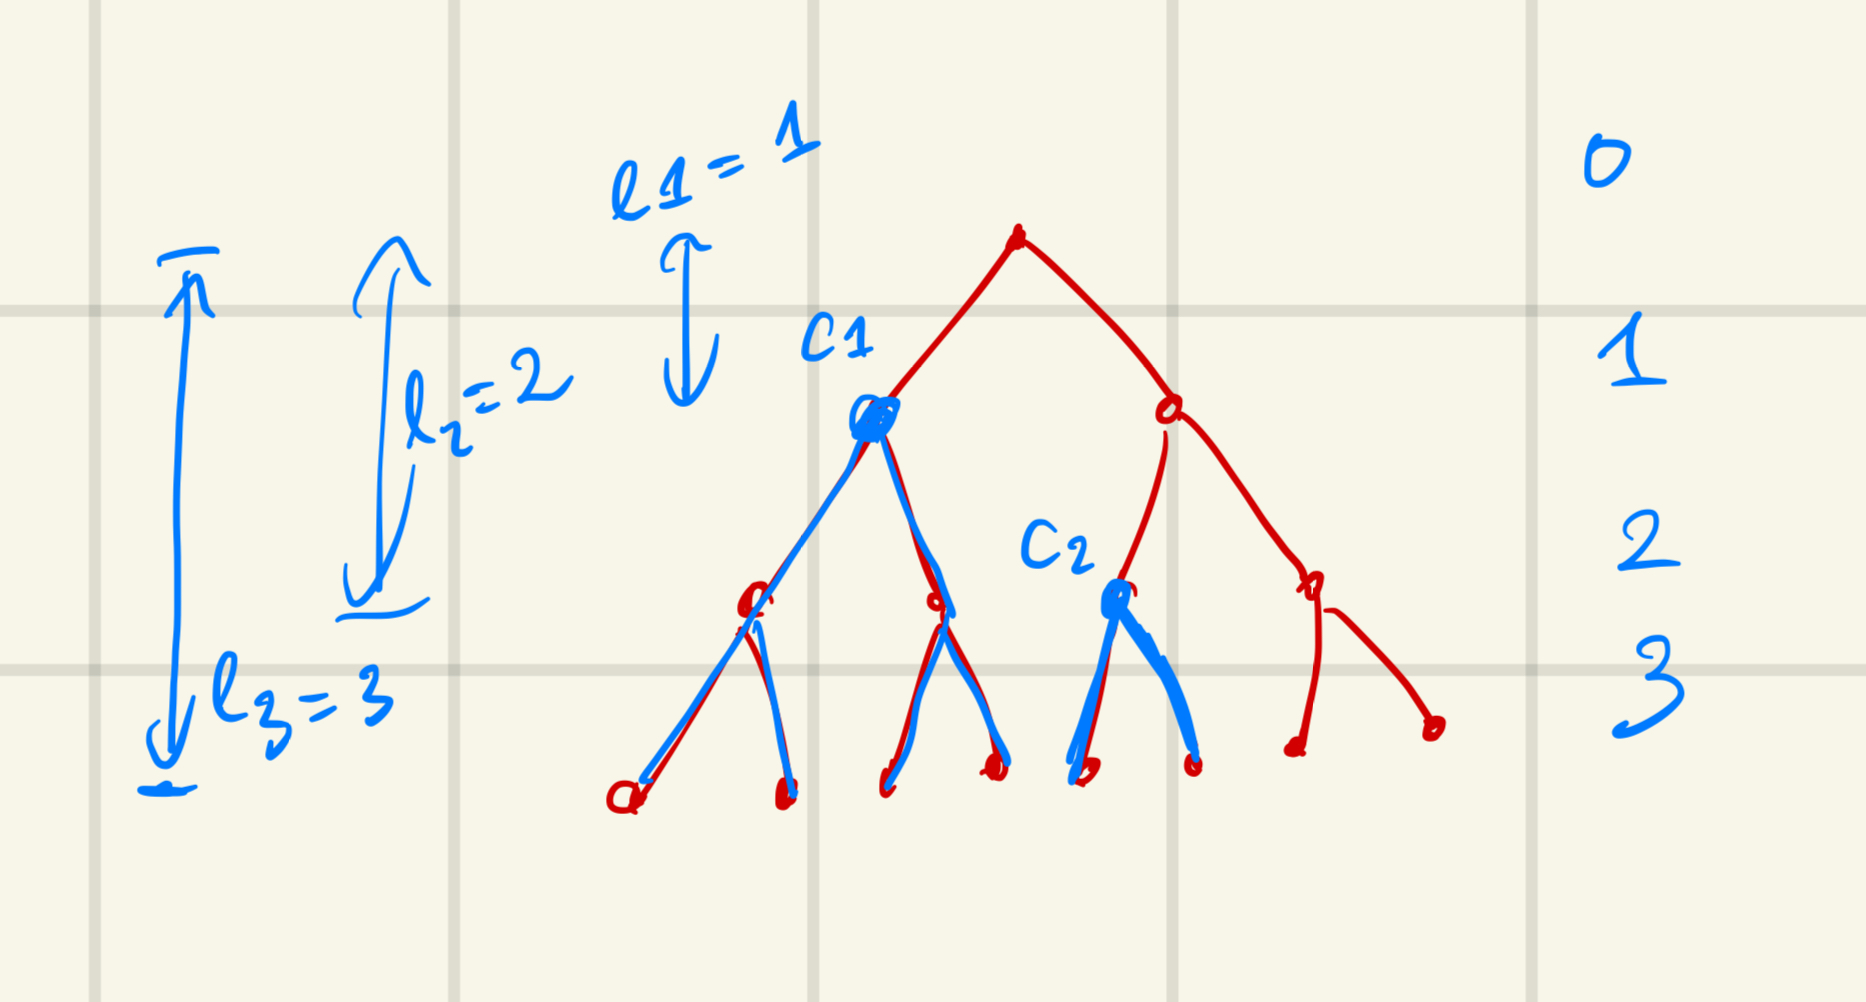
\includegraphics[width=0.5\textwidth]{btree.jpg}
\caption{binary tree}
\label{fig_btree}
\end{figure}

The code $C(i)$ of length $l_i$ occupies $2^{l_M - l_i}$ leaves, as $M-1$ code words is PF, then number of occupied leaves is
$$
    \sum_{i=1}^{M-1} 2^{l_M - l_i}
$$

Uniformly sample $C(M)$ is equivalent to uniformly pick from $2^{l_M}$ leaves, then probability of $C(M)$ being PF with the rest is

$$
    \frac{2^{l_M} - \sum_{i=1}^{M-1} 2^{l_M - l_i}}{2^{l_M}}  = 1 - \sum_{i = 1}^{M-1} 2^{-l_i}
$$

Let $E_M$ be the event the first $M$ code words being PF, we have

$$
    \frac{P(E_M)}{P(E_{M-1})} = \frac{P(E_M \cap E_{M-1})}{P(E_{M-1})} = P(E_M | E_{M-1}) = 1 - \sum_{i = 1}^{M-1} 2^{-l_i}
$$

By induction, we have

$$
    P_M(good) = P(E_M) = \prod_{k=1}^M \tuple*{1 - \sum_{i = 1}^{k-1} 2^{-l_i}}
$$

This is true only for $P(E_i) > 0$ for all $1 \leq i \leq M-1$. When there exists $P(E_i) = 0$, let $N = \min_i \set{i \in [M]: P(E_i) = 0}$, the recurrence relation is true for all $1 \leq k \leq N$
$$
    \frac{P(E_k)}{P(E_{k-1})} = 1 - \sum_{i = 1}^{k-1} 2^{-l_i}
$$

and after that for all $N+1 \leq k \leq M$
$$
    1 - \sum_{i = 1}^{k-1} 2^{-l_i} < 0
$$

Hence, we can rewrite $P_M(good)$ by
$$
    P_M(good) = P(E_M) = \prod_{k=1}^M \tuple*{1 - \sum_{i = 1}^{k-1} 2^{-l_i}}^+
$$


\subsection{$P_M (good) > 0$ if and only if there exists a PF code for a source with alphabet size M}

TRUE

As $M$ and $l_1, l_2, ..., l_M$ are finite, total number of bits $N$ is \textbf{finite}, hence if there exists a PF code, probability of sampling that code is $P_M(good) \geq 2^{-N} > 0$. On the other hands, $P_M(good)$ is the sum of all good code probabilities, $P_M(good) > 0$ implies there exists a good code. The situation is different if the sample space is not finite.

\subsection{prove Kraft inequality}

$P_M (good) > 0$ implies $\tuple*{1 - \sum_{j=1}^{k-1} 2^{-l_j}}^+ > 0$ for all $k$. Take $k=M$, then 
$$
    1 - \sum_{j=1}^{M - 1} 2^{-l_j} > 0
$$

Now we increase the size of input to $2^n M$ and the new lengths so that there are $2^n$ copies of $l_i$ for each $i$, then there exists a PF code such that each old code word is replicated into $2^n$ copies, i.e
$$
    C(i) \mapsto b \oplus C(i)
$$

for every $b \in \set{0, 1}^n$. The new code is prefix-free and we have

$$
    1 - \frac{2^n - 1}{2^n} \sum_{j=1}^{M} 2^{-l_j} - \frac{1}{2^n} \sum_{j=1}^{M-1} 2^{-l_j} > 0
$$

Taking limit at $n \to \infty$ recovers the Kraft inequality.
\end{document}
